\documentclass[letterpaper,11pt]{article}
\usepackage{graphicx}
\usepackage{listings}
\usepackage[super]{nth}
\usepackage[hyphens]{url}
\usepackage{hyperref}
\usepackage{amsmath}
\usepackage[makeroom]{cancel}
\usepackage[table]{xcolor}
\usepackage{comment}
\usepackage[space]{grffile}
\usepackage{csvsimple}
\usepackage{longtable}
\usepackage{adjustbox}


\newcommand*{\srcPath}{../src}%

\lstset{
	basicstyle=\footnotesize,
	breaklines=true,
}

\begin{document}

\begin{titlepage}

\begin{center}

\Huge{Assignment 3}

\Large{CS 734:  Introduction to Information Retrieval}

\Large{Fall 2017}

\Large{Grant Atkins}

\Large Finished on \today

\end{center}

\end{titlepage}

\newpage


% =================================
% First question
% =================================
\section*{1}

\subsection*{Question}

\begin{verbatim}
6.1. Using the Wikipedia collection provided at the book website, create 
a sample of stem clusters by the following process:
    1. Index the collection without stemming.
    2. Identify the first 1,000 words (in alphabetical order) in the index.
    3. Create stem classes by stemming these 1,000 words and recording 
    which words become the same stem.
    4. Compute association measures (Dice?s coefficient) between all 
    pairs of stems in each stem class. Compute co-occurrence at the 
    document level.
    5. Create stem clusters by thresholding the association measure. 
    All terms that are still connected to each other form the clusters.

Compare the stem clusters to the stem classes in terms of size and the 
quality (in your opinion) of the groupings.
\end{verbatim}

\subsection*{Answer}

For this problem as well as other problems that used Galago it should be noted that I used Galago version 3.12 \cite{galago}. 
I also used the wiki-small html files as the input for the Galago search engine.

To handle the first two parts of this problem I decided to take advantage of the Galago search engine for indexing and sorting the index created by it.
I then used galago to dump the unique keys from its inverted index using the following command: 

\begin{center}
{\$ galago dump-keys index/postings $>$ dump-keys.csv }
\end{center}

Galago creates an inverted index and it should be noted that from the keys dumped there were sequences of different characters but not all of them were actually words but rather numbers or misspellings. 
To compensate for this I used a python library called Pyenchant \cite{pyenchant} to go through each and see if the the words were actually english and spelled correctly.
The code to complete this is in \textbf{spellcheck.py} shown in Listing \ref{lst:spellcheck}. 
This however still had numbers inside of it. 
To get to the english words starting with the letter `a` I skipped to line 8578 and took the next 1000 words saved this to a file named \textbf{top-1k-words.txt}.
 
 \lstinputlisting[frame=single,caption={Spellcheck code in python},label=lst:spellcheck,captionpos=b,numbers=left,showspaces=false,showstringspaces=false,basicstyle=\footnotesize]{\srcPath/spellcheck.py}

To stem each of the words in my list I used the NLTK python library \cite{nltk} and specifically the PorterStemmer function to stem each word.
I made a dictionary where each stem was a key and the stems then had an array of words that fell into that stem class and saved this to a json file named \textbf{stems.json}.
A small sample of this is shown in Figure \ref{fig:stemspic}.
I then used Galago again to find the document ids where the words had been used using the following Galago command:

\begin{center}
{\$ galago dump-index index/postings $>$ dump.csv }
\end{center}

I then merged the previous dictionary with the document ids found in this step so I could use it to find the co-occurrence and Dice's Coefficient as described below. 
The code to perform these steps is in the file named \textbf{stemmer.py}.

\begin{figure}[h]
\centering
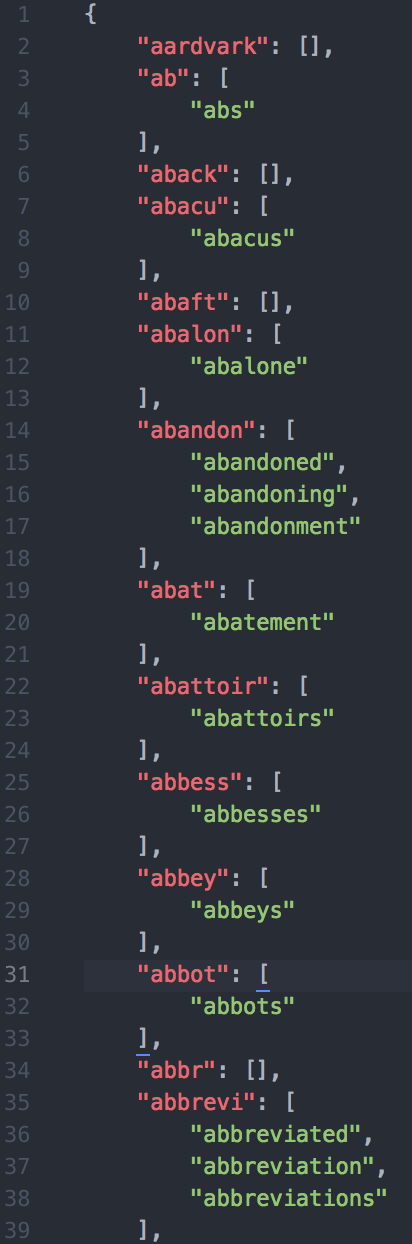
\includegraphics[scale=0.6]{stems.png}
\caption{Subset of stems generated from Porter Stemmer}
\label{fig:stemspic}
\end{figure}

Dice's Coefficient is described in our textbook \cite{book} as:

\[
    \frac{n_{ab}}{n_a+n_b}
\]

To compute Dice's Coefficient I used source code for the algorithm found en.wikibooks.org \cite{wikibook} and used the python version.
A subset of bigrams and their pair results of this are shown in Figure \ref{fig:dice}, saved in \textbf{dice.csv}.
The first column is the stem, the two words following are the comparisons, and the last value is the Dice Coefficient. 
The code used to create this is shown in Listing \ref{lst:dc}, written in diceCluster.py.

\begin{figure}[h]
\centering
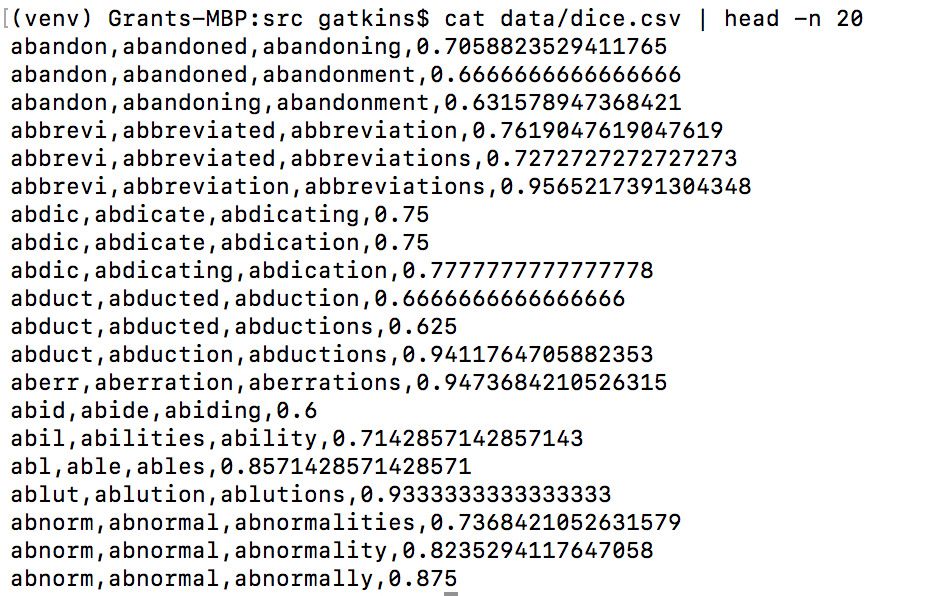
\includegraphics[scale=0.6]{dice.png}
\caption{Subset of stems, the bigram pairs, and the dice coefficients for each}
\label{fig:dice}
\end{figure}

Dice clusters were then calculated using:

\[
    \frac{2 * {doc\_count_{ab}}}{doc\_count_a+doc\_count_b}
\]

The threshold I set was 0.1 and I got a relatively high number of clusters, 100 as shown with a subset show in Figure \ref{fig:dicec}.
The difference is noticeable when comparing stem classes to stem clusters.
The influence of document frequency shows that this changes the cluster associations greatly.

\begin{figure}[h]
\centering
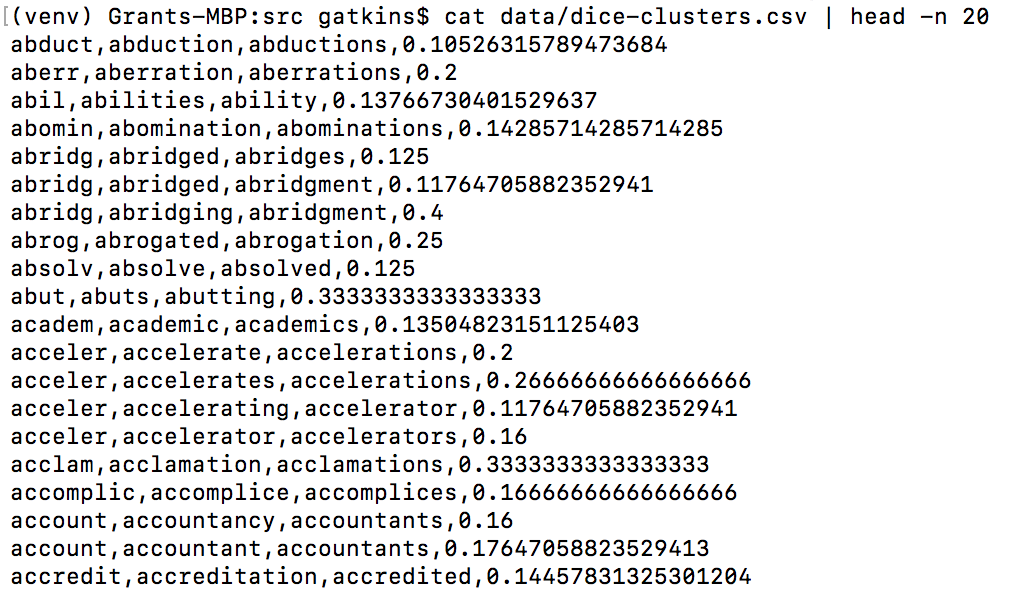
\includegraphics[scale=0.6]{dice-clusters.png}
\caption{Subset of stems, the bigram pairs, and the dice coefficients for each}
\label{fig:dicec}
\end{figure}

 \lstinputlisting[frame=single,caption={Code to compute Dice coefficient and clusters directory},label=lst:dc,captionpos=b,numbers=left,showspaces=false,showstringspaces=false,basicstyle=\footnotesize]{\srcPath/diceCluster.py}

\clearpage

% =================================
% Second question
% =================================

\section*{2}

\subsection*{Question}

\begin{verbatim}
6.4. Assuming you had a gazetteer of place names available, 
sketch out an algorithm for detecting place names or locations
in queries. Show examples of the types of queries where your 
algorithm would succeed and where it would fail.
\end{verbatim}

\subsection*{Answer}

When thinking of an algorithm for detecting places names or locations in queries two very simple solutions come to mind right away.
One is to tokenize the entire query and then search for each of the tokens directly in the index.
This solution is of course a can be time consuming especially if the index is very large.
Users never want to wait a long period of time because this method offers a slow solution.

Another simple solution is to have a cache of popular locations.
Whenever a query goes out it is again tokenized and then the terms can be searched inside a small cache to save time.
This however also has its own caveats of not covering every possible solution and actually increases time if it hits the cache first and doesn't find the location, but then also has to hit the index.

Another possible solution is to have predefined queries with modular variables in them.
Some of the possible queries and their interchangeable variables are:

\begin{itemize}
  \item ``I went to Vegas this Summer.'' -$>$ ``I went to X this Summer.''
  \item ``Washington and Virginia are almost the same.'' -$>$ ``X and Y are almost the same.''
\end{itemize}

These kinds of interchangeable queries could be stored procedures in a sense.
This approach could also be used for bigrams since these are based on positions.
This is a decent approach but there are many different ways to reference a location in a sentence therefore we can't contain cache of all the options.
If we conform other queries to these predefined queries it can introduce more false positives.
With this approach we also have to consider locations that aren't unigrams, such as ``North Carolina.''

An example algorithm is to combine each of these concepts into a single algorithm which updates overtime depending on the queries incoming.
The goal is to have an algorithm that can receive the advantages of these methods to increase query coverage, however there still might be locations that slip through each of these methods. My proposition is below in Listing \ref{lst:pseudo}.

\begin{lstlisting}[language=python, caption={Pseudo code algorithm for Location detection in queries}, label={lst:pseudo}]

// perform lookup for term - increment cache frequency regardless
function cache_lookup(query):
	if query in query_cache:
		query_cache[query] += 1
		return true
	else
		query_cache[query] += 1
		return false

// check predefined query templates - return list of locations
function check_templates(query):
	locations = []
	for temp in templates:
		if query like template:
			positions = template.location_positions
			for pos in positions:
				locations.append(query[pos])
			return locations
	return locations

// long lookup to index
function long_lookup(tokens):
	locations = []
	for t in tokens:
		if find_token_index(t):
			locations.append(t)
	return locations			
	
// function to execute by default
function find_locations(query):
	if cache_lookup(query):
		return location(s)
	else
		locations = check_templates(query)
		if length(locs) != 0:
			query_cache[query] += 1
			return locations
		else
			tokens = tokenize(query)
			locations = long_lookup(tokens)
			if length(locations) != 0:
				return locations
	// no location found at all
	return error_no_locations

find_locations(query);
\end{lstlisting}

This pseudo code go through each of the above stated methods and checks.
The order in which each executes should be the least costliest for each.
If no locations are found then it will return 0 or error message of ``no locations found.''
This algorithm also has an update policy to the cache for frequent queries.

\clearpage

% =================================
% 3rd question
% =================================

\section*{3}

\subsection*{Question}

\begin{verbatim}
7.7. What is the ``bucket'' analogy for a bigram language model?
Give examples.
\end{verbatim}

\subsection*{Answer}

In the bigram language model the ``bucket'' analogy is very similar to the analogy as unigrams as well.
In the unigram model the analogy of the ``bucket'' is the idea of reaching into an bucket of words for a document, reading off a word, and then putting it back in the bucket.
Its probabilistic that words with a high frequency or are important will be drawn more often than others.

The bigram model is very similar except for the fact that it retrieves two word pairs from a bucket which represents a document.
The two word pairs are words that are adjacent to one another in a document, therefore providing ordering of words.
These bigrams also provide more context than a unigram model since they provide this ordering. 
For example, the sentence ``North Carolina citizens wants to outlast the storm'' would be create the following list in a unigram language model:

\begin{itemize}
  \item ``North''
  \item ``Carolina''
  \item ``citizens''
  \item ``wants''
  \item ``outlast''
  \item ``storm''
\end{itemize}

This has all of the stop word removed but these words become representative of the document that are in.
In the bigram language model the following list would be created from the previous list:

\begin{itemize}
  \item ``North Carolina''
  \item ``Carolina citizens''
  \item ``citizens wants''
  \item ``wants outlast''
  \item ``outlast storm''
\end{itemize}

If a user picks out the word ``North'' from the unigram bucket it proves to be a very ambiguous word.
However, if we pick out the first bigram which contains ``North'' it becomes ``North Carolina.''
This brings a lot more context as well shows connections between words.
The frequency of the these word pairs will prove to be a better representative of the document than that of the unigrams.
This also shows that the second word of the bigrams are dependent on the first word.
As the occurrences of bigrams starting with ``North'' increase whichever second word for the bigram starts to become more representative for the distribution.
So if there are two ``North Carolina'' occurrences its apparent that this has more weight over one ``North Virginia'' occurrence to represent a document.

% \lstinputlisting[frame=single,caption={Sitemap created from my assignment 1 (A1) directory},label=lst:sitemap_output,captionpos=b,numbers=left,showspaces=false,showstringspaces=false,basicstyle=\footnotesize]{\srcPath/data/sitemap.xml}

\clearpage

% =================================
% 4th question
% =================================

\section*{4}

\subsection*{Question}

\begin{verbatim}

\end{verbatim}

\subsection*{Answer}




\clearpage

% =================================
% 5th question
% =================================

\section*{5}

\subsection*{Question}

\begin{verbatim}

\end{verbatim}

\subsection*{Answer}


\clearpage


\clearpage


% =================================
% Bibliography
% =================================

\begin{thebibliography}{9}
\bibitem{github}
Atkins, Grant. ``CS734 Assignment 3 Repository'' Github. N.p., 9 November 2017. Web. 9 November 2017.\url{https://github.com/grantat/cs834-f17/tree/master/assignments/A3}.
\bibitem{book}
B. Croft, D. Metzler, and T. Strohman. ``Search Engines: Information Retrieval in Practice.'' Pearson, 2009. Web. 14 October 2017. ISBN 9780136072249.
\bibitem{nltk}
Bird, Steven, Edward Loper and Ewan Klein (2009). ``Natural Language Processing with Python`` O?Reilly Media Inc. Web. 9 November 2017.\url{http://www.nltk.org/}.
\bibitem{galago}
``The Lemur Project - Galago''. Web. 9 November 2017. \url{https://sourceforge.net/p/lemur/wiki/Galago/}.
\bibitem{pyenchant}
``Pyenchant''. Web. 9 November 2017. \url{http://pythonhosted.org/pyenchant/}.
\bibitem{wikibook}
``Wikibook - Dice's Coefficient''. Web. 9 November 2017. \url{https://en.wikibooks.org/wiki/Algorithm_Implementation/Strings/Dice%27s_coefficient#Python}.
\end{thebibliography}

\end{document}
